% !TeX program = lualatex
% ================================================================
% Polish Tier 3 Vocabulary Version of AppliedRatioCrossTopics
%
% Generated by the server using the following settings:
%
%   language            Polish (pol)
%   text direction      left to right
%   font                Noto Serif
%   fallback font       Noto Serif
%   built from          latex/worksheets/ratioAndProportion/crossTopic/appliedRatioCrossTopics.tex
%   vocabulary key      latex/worksheets/ratioAndProportion/crossTopic/appliedRatioCrossTopics/L2/pol/appliedRatioCrossTopics_polishKey.tex
%   tier 3 vocabulary   green   RGB 0 128 0
%   English text        black   RGB 0 0 0
%   Polish text         purple  RGB 112 48 160
%   layout macros       version 3
%
% Please don't edit any information in this comment block - the server
% compares it against the current settings and rebuilds this file when
% they differ, so changes here would be overwritten. However, feel free
% to make updates to the LaTeX below if you want to edit it.
% ================================================================

\documentclass[12pt]{article}
% ================================================================
% Copied from the English sheet this was translated from, so that
% anything it sets up for itself still works here
% ================================================================
\usepackage{amsmath}
\usepackage{tikz}
\usepackage{enumitem}
\usepackage[margin=1in]{geometry}

\title{Applied Ratio Extension Problems}
\date{}

% Characters this language's font has not got are borrowed from another,
% rather than being silently dropped - see docs/translated-sheet-latex.md
\directlua{%
  if luaotfload and luaotfload.add_fallback then
    luaotfload.add_fallback("eallatinfallback",
      { "Noto Serif:mode=harf;" })
  else
    tex.error("this luaotfload is too old to register a fallback font")
  end
}
\usepackage[english]{babel}
\babelprovide[import]{polish}
\babelfont[polish]{rm}[Renderer=Harfbuzz, BoldFont={Noto Serif}, ItalicFont={Noto Serif}, BoldItalicFont={Noto Serif}, RawFeature={fallback=eallatinfallback}]{Noto Serif}
\babelfont[polish]{sf}[Renderer=Harfbuzz, BoldFont={Noto Serif}, ItalicFont={Noto Serif}, BoldItalicFont={Noto Serif}, RawFeature={fallback=eallatinfallback}]{Noto Serif}
\newcommand{\ealtext}[1]{\foreignlanguage{polish}{#1}}
\newcommand{\ealtextblock}[1]{{\raggedright\foreignlanguage{polish}{#1}\par}}
% ================================================================
% EAL layout helpers
% ================================================================
\usepackage{xcolor}

\definecolor{ealkeycolour}{RGB}{0,128,0}
\definecolor{ealenglish}{RGB}{0,0,0}
\definecolor{ealtwocolour}{RGB}{112,48,160}

\newsavebox{\ealboxen}
\newsavebox{\ealboxtr}
\newlength{\ealglosswd}
\newlength{\ealglossraise}
\setlength{\ealglossraise}{1.15em}

% a tier 3 word, in English and in translation alike
\newcommand{\ealkey}[1]{\textcolor{ealkeycolour}{#1}}
\newcommand{\ealkeytr}[1]{\textcolor{ealkeycolour}{\ealtext{#1}}}

% One translated word above one English word. Built from kernel
% primitives, never a tabular, which would break wherever the sheet
% loads array, booktabs or tabularx. The box is as wide as the wider of
% the two, so a long translation pushes its neighbours aside instead of
% overlapping them, and it claims its full height so a table row or a
% TikZ node makes room for it.
\newcommand{\ealgloss}[2]{%
  \sbox{\ealboxen}{\ealkey{#1}}%
  \sbox{\ealboxtr}{\small\textcolor{ealtwocolour}{\ealtext{#2}}}%
  \setlength{\ealglosswd}{\wd\ealboxen}%
  \ifdim\wd\ealboxtr>\ealglosswd\setlength{\ealglosswd}{\wd\ealboxtr}\fi
  \leavevmode
  \makebox[\ealglosswd][c]{%
    \makebox[0pt][c]{\usebox{\ealboxen}}%
    \makebox[0pt][c]{\raisebox{\ealglossraise}{\usebox{\ealboxtr}}}%
  }%
}

% opens up line spacing around a block of glosses, so the raised
% translations sit clear of the line above
\newenvironment{ealglossed}{\par\linespread{2.1}\selectfont\ignorespaces}{\par}

% a whole translated sentence above its English counterpart. block level,
% so it does not belong inside a tabular cell
\newcommand{\ealpara}[2]{%
  \par\addvspace{0.5\baselineskip}%
  {\color{ealtwocolour}\ealtextblock{#1}}%
  \penalty200
  {\color{ealenglish}#2\par}%
  \addvspace{0.5\baselineskip}%
}

\begin{document}

\maketitle

\section*{Recipe Questions Past}

\begin{enumerate}
\item A muffin recipe makes 12 muffins with the following ingredients:
    \begin{itemize}
    \item 300g flour
    \item 200g sugar
    \item 2 eggs (approx. 100g)
    \item 250ml milk
    \end{itemize}
    You want to increase the yield by 50\%. Calculate the new quantities for all ingredients.

\item A sauce recipe serves 4 people:
    \begin{itemize}
    \item 400ml tomato passata
    \item 2 cloves garlic (20g)
    \item 100ml olive oil
    \item 50g fresh basil
    \end{itemize}
    You only want to make 75\% of the original recipe. Calculate the new quantities.

\item A cake recipe that serves 6 people requires:
    \begin{itemize}
    \item 240g flour
    \item 180g butter
    \item 150g sugar
    \item 3 eggs (150g)
    \end{itemize}
    \begin{ealglossed}
    You need to serve 10 people. By what \ealgloss{percentage}{procent} must you increase the recipe? Calculate all new ingredient quantities.
    \end{ealglossed}

\item \begin{ealglossed}
After cooking, you have 560g of pasta from a recipe that was increased by 40\% from its original size. What was the original \ealgloss{mass}{masa} of pasta the recipe made?
\end{ealglossed}

\newpage{}

\item A bread recipe uses:
    \begin{itemize}
    \item 1000g flour
    \item 600ml water
    \item 20g salt
    \item 15g yeast
    \end{itemize}
    The baker makes a new batch using 850g of flour after reducing the recipe.
    \begin{enumerate}
    \item \begin{ealglossed}By what \ealgloss{percentage}{procent} was the recipe reduced?\end{ealglossed}
    \item Calculate the new quantities for all other ingredients.
    \end{enumerate}
\end{enumerate}


\section*{Recipe Questions Future}

\begin{enumerate}[resume]
\item You are making a square brownie. The recipe for a 20cm × 20cm tray uses:
    \begin{itemize}
    \item 200g chocolate
    \item 150g butter
    \item 3 eggs
    \end{itemize}
    You are using a larger 25cm × 25cm tray. Calculate the new quantities for all ingredients.

\item \begin{ealglossed}
You are baking a circular cake. The original recipe is for a cake tin with a \ealgloss{diameter}{średnica} of 20cm and uses:
    \begin{itemize}
    \item 250g flour
    \item 200g sugar
    \item 4 eggs
    \end{itemize}
    You are using a tin with a \ealgloss{diameter}{średnica} of 30cm. Calculate the new quantities.
\end{ealglossed}

\item \begin{ealglossed}
You are making two rectangular pizzas. The large pizza has \ealgloss{dimensions}{wymiary} 35cm × 25cm. The small pizza has \ealgloss{dimensions}{wymiary} 20cm × 15cm. The small pizza recipe uses:
    \begin{itemize}
    \item 200g cheese
    \item 150g flour
    \item 100ml tomato sauce
    \end{itemize}
    \begin{enumerate}
    \item What is the \ealgloss{area}{pole} of each pizza?
    \item How much of each ingredient does the large pizza need?
    \end{enumerate}
\end{ealglossed}

\newpage{}

\item \begin{ealglossed}
You are decorating the \ealgloss{perimeter}{obwód} of a rectangular cake with sprinkles. The cake is 28cm long and 18cm wide. One gram of sprinkles covers 4cm of \ealgloss{perimeter}{obwód}.
    \begin{itemize}
    \item 300g cake base
    \item 200g icing
    \item 50g sprinkles (original amount)
    \end{itemize}
    \begin{enumerate}
    \item What is the \ealgloss{perimeter}{obwód} of your cake?
    \item How many grams of sprinkles do you need?
    \item If you make a cake with double the \ealgloss{perimeter}{obwód}, by what \ealgloss{factor}{dzielnik} should you multiply all ingredients?
    \end{enumerate}
\end{ealglossed}

\item \begin{ealglossed}
A fancy triangular dessert has side lengths 12cm, 12cm, and 8cm. You create a \ealgloss{similar}{podobny} dessert where all side lengths are increased by a \ealgloss{scale factor}{współczynnik skali} of 1.5.
\end{ealglossed}
\begin{center}
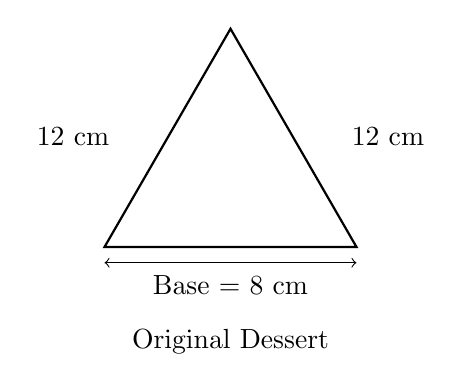
\begin{tikzpicture}[scale=0.4]
\draw[thick] (0,0) -- (8,0) -- (4,6.928) -- cycle;
\node at (4, -1.2) {Base = 8 cm};
\node at (9, 3.5) {12 cm};
\node at (-1, 3.5) {12 cm};
\draw[<->] (0,-0.5) -- (8,-0.5);
\node at (4, -3) {Original Dessert};
\end{tikzpicture}
\end{center}

    \begin{ealglossed}
    The original recipe uses:
    \begin{itemize}
    \item 120g sugar (for the \ealgloss{area}{pole})
    \item 80g cocoa powder (for the \ealgloss{perimeter}{obwód} decoration)
    \item 3 eggs
    \end{itemize}
    \end{ealglossed}
    \begin{ealglossed}
    \begin{enumerate}
    \item What is the \ealgloss{perimeter}{obwód} of the original dessert?
    \item What is the \ealgloss{perimeter}{obwód} of the new, larger dessert?
    \item How much sugar is needed for the larger dessert?
    \item How much cocoa powder is needed for the larger dessert?
    \item How many eggs are needed for the larger dessert?
    \end{enumerate}
    \end{ealglossed}
\end{enumerate}

\newpage{}

\section*{Best Buys Past}

\begin{enumerate}[resume]
\item A 500g box of cereal costs £4.50. A 750g box costs £6.30. Which is the better buy?

\item Store A sells 6 cans of soda for \$4.80. Store B sells the same soda with a 15\% discount on single cans that normally cost \$0.95 each. Where should you buy if you need 6 cans?

\item A 2L bottle of juice costs €3.20. The 1.5L bottle is on sale for 20\% off its regular price of €2.80. Which size offers better value per liter?

\item \textbf{Electronic World} is having a clearance sale: \\
Headphones: Original £120, now 20\% off \\
Speakers: Original £85, now 30\% off \\ \\
The store is also running a buy 3 items, get the cheapest free deal. You can sell electronics for 50\% of non-discounted price to a local shop - what is the cheapest way you can buy both the headphones and speakers?

\item \begin{ealglossed}
A furniture store offers two payment plans for a £1200 sofa: \\
Plan A: 25\% down payment, then 12 monthly payments of £80 \\
Plan B: No down payment, 18 monthly payments of £75 \\
Considering the total amount paid, which plan is better and by what \ealgloss{percentage}{procent} of the original price?
\end{ealglossed}
\end{enumerate}

\vspace{2cm}

\section*{Best Buys Future}

\begin{enumerate}[resume]
\item You need to fence a rectangular garden. Store A sells fencing for \$12 per meter. Store B sells pre-cut 2m sections for \$20 each. Which is cheaper for a 10m × 8m garden?

\item You want to tile a floor. Tile Type A costs £25 per square meter. Tile Type B costs £18 per square meter but requires 15\% more tiles due to breakage. For a 4m × 5m room, what is the lowest price to tile the room?

\item \begin{ealglossed}
Paint costs £35 per liter and covers 12m² per liter. Brand X offers 20\% more coverage per liter for £42 per liter. For painting two walls of \ealgloss{dimensions}{wymiary} 4m × 3m and 5m × 3m, which paint is better value? Buying the cheapest, how much will the paint cost?
\end{ealglossed}

\newpage{}

\item \begin{ealglossed}
You need to buy grass seed for a lawn. The lawn consists of a rectangle (10m × 6m) with a \ealgloss{semicircular}{półkoliste} extension (\ealgloss{radius}{promień} 3m) at one end. Seed A covers 15m² per kg at \$4.80 per kg. Seed B covers 25m² per kg at \$7.50 per kg. Which seed is more economical?
\end{ealglossed}

\begin{center}
\begin{tikzpicture}[scale=0.7]
\draw (0,0) rectangle (10,6);
\draw (10,0) arc (-90:90:3 and 3);
\draw (10,3) -- (10,0);
\node at (5,-0.5) {10m};
\node at (9.5 ,3) {6m};
\end{tikzpicture}
\end{center}

\item \begin{ealglossed}
A swimming pool has the following shape: a central rectangle 8m × 4m, with \ealgloss{semicircular}{półkoliste} ends of \ealgloss{radius}{promień} 2m. You need to buy a pool cover. Material X costs \$18 per m² and lasts 3 years. Material Y costs \$25 per m² and lasts 5 years. Considering cost per year, which material is more economical? How much will it cost per year to keep the pool covered for the least price?
\end{ealglossed}

\begin{center}
\begin{tikzpicture}[scale=0.7]
\draw (0,0) -- (8,0);
\draw (0,4) -- (8,4);
\draw (0,0) arc (-90:90:2 and 2);
\draw (8,0) arc (-90:-270:2 and 2);
\node at (4,-0.5) {8m};
\node at (9,2) {4m};
\end{tikzpicture}
\end{center}

\end{enumerate}

\newpage{}


\section*{Scaling Past}

\begin{enumerate}[resume]

\item \begin{ealglossed}
A drawing is \ealgloss{scaled}{skalowany} up by 150\%. If the original length was 8 cm, what is the new length?
\end{ealglossed}

\item \begin{ealglossed}
A map \ealgloss{scale}{skalować} is 1:25,000. What \ealgloss{percentage}{procent} of the actual distance does 1 cm on the map represent?
\end{ealglossed}

\item A photo is reduced to 80\% of its original size. If the reduced width is 12 cm, what was the original width?

\item \begin{ealglossed}
Sarah is creating a \ealgloss{scale}{skalować} drawing of her bedroom. She decides to use a \ealgloss{scale}{skalować} which represents 2\% of actual size. What \ealgloss{ratio}{stosunek} represents here \ealgloss{scale}{skalować}? If her bed measures 2 meters long in reality, what length should she draw it in her \ealgloss{scale}{skalować} drawing? Give your answer in centimetres.
\end{ealglossed}

\item \begin{ealglossed}
A company is producing \ealgloss{scale}{skalować} models of buildings. Model A is made at 2.5\% of actual size, while Model B is made at 4\% of actual size. 
\begin{enumerate}
    \item If a window is 1.2 meters wide in the actual building, how wide is it in each model?
    \item If Model A's height is 45 cm, what is the actual building's height?
    \item What \ealgloss{percentage}{procent} larger is Model B compared to Model A?
\end{enumerate}
\end{ealglossed}

\end{enumerate}


\section*{Scaling Future}

\begin{enumerate}[left=0pt, start=11]

\item \begin{ealglossed}
A square is enlarged using \ealgloss{scale factor}{współczynnik skali} 3. If the original \ealgloss{perimeter}{obwód} was 12 cm, what is the new \ealgloss{perimeter}{obwód}?
\end{ealglossed}

\item \begin{ealglossed}
A \ealgloss{scale}{skalować} drawing of a rectangular field uses \ealgloss{scale}{skalować} 1:200. If the drawing shows the field as 6 cm × 4 cm, what is the actual \ealgloss{area}{pole} of the field?
\end{ealglossed}

\begin{ealglossed}
The \ealgloss{equilateral triangle}{trójkąt równoboczny} below represents a park. If each side $s$ is 2 cm in the drawing, find:
\end{ealglossed}
\begin{ealglossed}
\begin{enumerate}
    \item The actual \ealgloss{perimeter}{obwód} of the park
    \item The actual \ealgloss{area}{pole} of the park (\ealgloss{area}{pole} of \ealgloss{equilateral triangle}{trójkąt równoboczny} = $\frac{\sqrt{3}}{4}s^2$)
\end{enumerate}
\end{ealglossed}

\begin{center}
\item 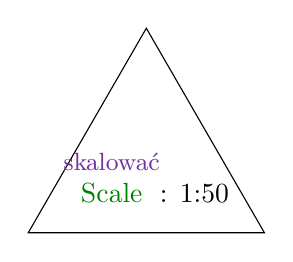
\begin{tikzpicture}[scale=0.5]
\draw (0,0) -- (6,0) -- (3,5.196) -- cycle;
\node at (3,1.4) {\ealgloss{Scale}{skalować}: 1:50};
\end{tikzpicture}
\end{center}

\newpage{}

\item \begin{ealglossed}
A blueprint shows a circular fountain with \ealgloss{diameter}{średnica} 3 cm at \ealgloss{scale}{skalować} 1:30. 
\begin{enumerate}
    \item What is the actual \ealgloss{diameter}{średnica} of the fountain?
    \item Calculate the actual \ealgloss{area}{pole} of the fountain's surface.
    \item If the \ealgloss{scale}{skalować} was changed to 1:45, what would be the drawn \ealgloss{diameter}{średnica}?
\end{enumerate}
\end{ealglossed}

\item \begin{ealglossed}
An architect creates \ealgloss{scale}{skalować} drawings of two \ealgloss{similar}{podobne} rectangular rooms. Room A is drawn at \ealgloss{scale}{skalować} 1:100 and measures 5 cm × 4 cm in the drawing. Room B is drawn at \ealgloss{scale}{skalować} 1:80 and measures 6 cm × ? cm in the drawing.
\begin{enumerate}
    \item Calculate the actual \ealgloss{dimensions}{wymiary} and \ealgloss{area}{pole} of each room.
    \item Which room has the larger actual \ealgloss{area}{pole} and by what \ealgloss{percentage}{procent}?
    \item If both drawings were converted to \ealgloss{scale}{skalować} 1:50, what would be their new \ealgloss{dimensions}{wymiary} on paper?
\end{enumerate}
\end{ealglossed}

\end{enumerate}

\end{document}